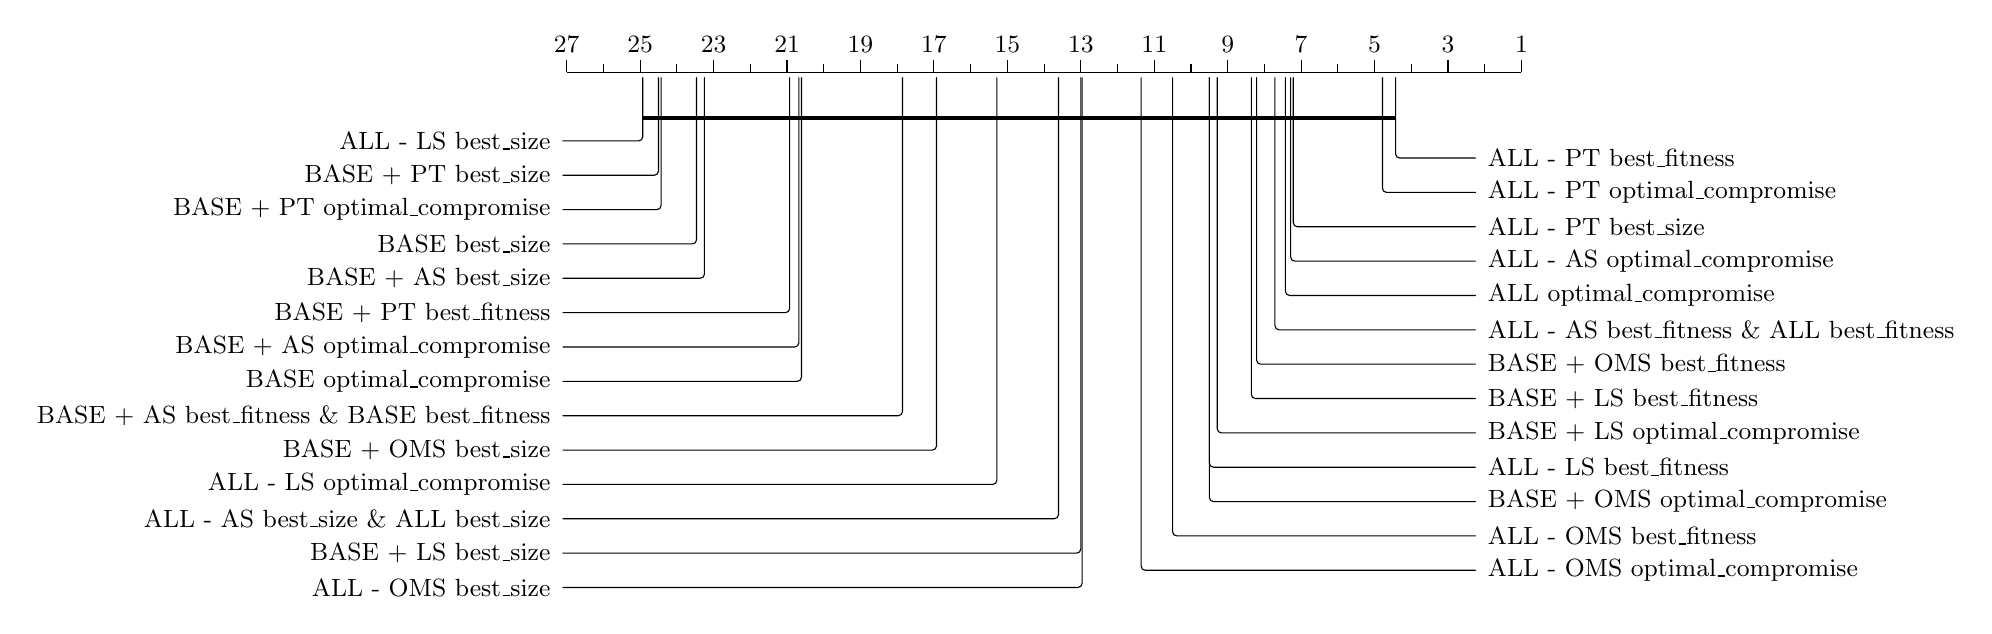
\begin{tikzpicture}[
  treatment line/.style={rounded corners=1.5pt, line cap=round, shorten >=1pt},
  treatment label/.style={font=\small},
  group line/.style={ultra thick},
]

\begin{axis}[
  clip={false},
  axis x line={center},
  axis y line={none},
  axis line style={-},
  xmin={1},
  ymax={0},
  scale only axis={true},
  width={\linewidth},
  ticklabel style={anchor=south, yshift=1.3*\pgfkeysvalueof{/pgfplots/major tick length}, font=\small},
  every tick/.style={draw=black},
  major tick style={yshift=.5*\pgfkeysvalueof{/pgfplots/major tick length}},
  minor tick style={yshift=.5*\pgfkeysvalueof{/pgfplots/minor tick length}},
  title style={yshift=\baselineskip},
  xmax={27},
  ymin={-14.5},
  height={15\baselineskip},
  xtick={1,3,5,7,9,11,13,15,17,19,21,23,25,27},
  minor x tick num={1},
  x dir={reverse},
]

\draw[treatment line] ([yshift=-2pt] axis cs:4.428571428571429, 0) |- (axis cs:2.178571428571429, -2.5)
  node[treatment label, anchor=west] {ALL - PT best\_fitness};
\draw[treatment line] ([yshift=-2pt] axis cs:4.785714285714286, 0) |- (axis cs:2.178571428571429, -3.5)
  node[treatment label, anchor=west] {ALL - PT optimal\_compromise};
\draw[treatment line] ([yshift=-2pt] axis cs:7.214285714285714, 0) |- (axis cs:2.178571428571429, -4.5)
  node[treatment label, anchor=west] {ALL - PT best\_size};
\draw[treatment line] ([yshift=-2pt] axis cs:7.285714285714286, 0) |- (axis cs:2.178571428571429, -5.5)
  node[treatment label, anchor=west] {ALL - AS optimal\_compromise};
\draw[treatment line] ([yshift=-2pt] axis cs:7.428571428571429, 0) |- (axis cs:2.178571428571429, -6.5)
  node[treatment label, anchor=west] {ALL optimal\_compromise};
\draw[treatment line] ([yshift=-2pt] axis cs:7.714285714285714, 0) |- (axis cs:2.178571428571429, -7.5)
  node[treatment label, anchor=west] {ALL - AS best\_fitness \& ALL best\_fitness};
\draw[treatment line] ([yshift=-2pt] axis cs:8.214285714285714, 0) |- (axis cs:2.178571428571429, -8.5)
  node[treatment label, anchor=west] {BASE + OMS best\_fitness};
\draw[treatment line] ([yshift=-2pt] axis cs:8.357142857142858, 0) |- (axis cs:2.178571428571429, -9.5)
  node[treatment label, anchor=west] {BASE + LS best\_fitness};
\draw[treatment line] ([yshift=-2pt] axis cs:9.285714285714286, 0) |- (axis cs:2.178571428571429, -10.5)
  node[treatment label, anchor=west] {BASE + LS optimal\_compromise};
\draw[treatment line] ([yshift=-2pt] axis cs:9.5, 0) |- (axis cs:2.178571428571429, -11.5)
  node[treatment label, anchor=west] {ALL - LS best\_fitness};
\draw[treatment line] ([yshift=-2pt] axis cs:9.5, 0) |- (axis cs:2.178571428571429, -12.5)
  node[treatment label, anchor=west] {BASE + OMS optimal\_compromise};
\draw[treatment line] ([yshift=-2pt] axis cs:10.5, 0) |- (axis cs:2.178571428571429, -13.5)
  node[treatment label, anchor=west] {ALL - OMS best\_fitness};
\draw[treatment line] ([yshift=-2pt] axis cs:11.357142857142858, 0) |- (axis cs:2.178571428571429, -14.5)
  node[treatment label, anchor=west] {ALL - OMS optimal\_compromise};
\draw[treatment line] ([yshift=-2pt] axis cs:12.964285714285714, 0) |- (axis cs:27.178571428571427, -15.0)
  node[treatment label, anchor=east] {ALL - OMS best\_size};
\draw[treatment line] ([yshift=-2pt] axis cs:13.0, 0) |- (axis cs:27.178571428571427, -14.0)
  node[treatment label, anchor=east] {BASE + LS best\_size};
\draw[treatment line] ([yshift=-2pt] axis cs:13.607142857142858, 0) |- (axis cs:27.178571428571427, -13.0)
  node[treatment label, anchor=east] {ALL - AS best\_size \& ALL best\_size};
\draw[treatment line] ([yshift=-2pt] axis cs:15.285714285714286, 0) |- (axis cs:27.178571428571427, -12.0)
  node[treatment label, anchor=east] {ALL - LS optimal\_compromise};
\draw[treatment line] ([yshift=-2pt] axis cs:16.928571428571427, 0) |- (axis cs:27.178571428571427, -11.0)
  node[treatment label, anchor=east] {BASE + OMS best\_size};
\draw[treatment line] ([yshift=-2pt] axis cs:17.857142857142858, 0) |- (axis cs:27.178571428571427, -10.0)
  node[treatment label, anchor=east] {BASE + AS best\_fitness \& BASE best\_fitness};
\draw[treatment line] ([yshift=-2pt] axis cs:20.607142857142858, 0) |- (axis cs:27.178571428571427, -9.0)
  node[treatment label, anchor=east] {BASE optimal\_compromise};
\draw[treatment line] ([yshift=-2pt] axis cs:20.678571428571427, 0) |- (axis cs:27.178571428571427, -8.0)
  node[treatment label, anchor=east] {BASE + AS optimal\_compromise};
\draw[treatment line] ([yshift=-2pt] axis cs:20.928571428571427, 0) |- (axis cs:27.178571428571427, -7.0)
  node[treatment label, anchor=east] {BASE + PT best\_fitness};
\draw[treatment line] ([yshift=-2pt] axis cs:23.25, 0) |- (axis cs:27.178571428571427, -6.0)
  node[treatment label, anchor=east] {BASE + AS best\_size};
\draw[treatment line] ([yshift=-2pt] axis cs:23.464285714285715, 0) |- (axis cs:27.178571428571427, -5.0)
  node[treatment label, anchor=east] {BASE best\_size};
\draw[treatment line] ([yshift=-2pt] axis cs:24.428571428571427, 0) |- (axis cs:27.178571428571427, -4.0)
  node[treatment label, anchor=east] {BASE + PT optimal\_compromise};
\draw[treatment line] ([yshift=-2pt] axis cs:24.5, 0) |- (axis cs:27.178571428571427, -3.0)
  node[treatment label, anchor=east] {BASE + PT best\_size};
\draw[treatment line] ([yshift=-2pt] axis cs:24.928571428571427, 0) |- (axis cs:27.178571428571427, -2.0)
  node[treatment label, anchor=east] {ALL - LS best\_size};
\draw[group line] (axis cs:4.428571428571429, -1.3333333333333333) -- (axis cs:24.928571428571427, -1.3333333333333333);

\end{axis}
\end{tikzpicture}